% % % % % % % % % % % % % % % % % % % % % % % % % % % % % % % % % % % % % % % % % % % %
%                                                                                     %
% Short Sectioned Assignment LaTeX Template Version 1.0 (5/5/12)                      %
% This template has been downloaded from: http://www.LaTeXTemplates.com               %
%                                                                                     %
% Original author:  Frits Wenneker (http://www.howtotex.com)                          %
%                                                                                     %
% Modified by: Fco Javier Sueza Rodríguez (fcosueza@disroot.org)                      %
%                                                                                     %
% Changes:                                                                            %
%	    - Custom Chapters, Sections and Subsections (titlesec package)                %
%           - Document type scrbook (oneside)                                         %
%           - Use babel-lang-spanish package and marvosym                             %
%           - Use hyperref, enumitem, tcolorbox and glossaries packages               %
%           - Use Time New Roman (mathptmx), Helvetic and Courier fonts               %
%                                                                                     %
% License: CC BY-NC-SA 3.0 (http://creativecommons.org/licenses/by-nc-sa/3.0/)        %
%                                                                                     %
% % % % % % % % % % % % % % % % % % % % % % % % % % % % % % % % % % % % % % % % % % % %

%-----------------------------------------------%
%	              Packages                  %
%-----------------------------------------------%

\documentclass[paper=a4, fontsize=11pt, oneside]{scrbook}

% ---- Text Input/Output ----- %

\usepackage[T1]{fontenc}
\usepackage[utf8]{inputenc}
\usepackage{mathptmx}
\usepackage[scaled=.92]{helvet}
\usepackage{courier}
\usepackage[indent=12pt]{parskip}

\usepackage{geometry}
\geometry{verbose,tmargin=3cm,bmargin=3cm,lmargin=2.6cm,rmargin=2.6cm}

% ---- Language ----- %

\usepackage[spanish]{babel}
\usepackage{marvosym}

% ---- Another packages ---- %

\usepackage{amsmath,amsfonts,amsthm}
\usepackage{graphics,graphicx}
\usepackage{titlesec}
\usepackage{fancyhdr}
\usepackage{tcolorbox}
\usepackage{hyperref}
\usepackage{enumitem}
\usepackage[automake]{glossaries}

%--------------------------------------------------------------------%
%                      Customizing Document                          %
%--------------------------------------------------------------------%


% ----------- Custom Chapters, Sections and Subsections -------------- %

\titleformat{\chapter}[display]
			{\bfseries\Huge}
			{Tema \ \thechapter} {0.5ex}
			{\vspace{1ex}\centering}

\titleformat{\section}[hang]
			{\bfseries\Large}
			{\thesection}{0.5em}{}

\titleformat{\subsection}[hang]
			{\bfseries\large}
			{\thesubsection}{0.5em}{}

\titleformat{\subsubsection}[hang]
			{\bfseries\large}
			{\thesubsubsection}{0.5em}{}

\hypersetup{
    colorlinks=true,
    linkcolor=black,
    urlcolor=magenta
}

% ------------------- Custom heaaders and footers ------------------- %

\pagestyle{fancyplain}

\fancyhead[]{}
\fancyfoot[L]{}
\fancyfoot[C]{}
\fancyfoot[R]{\thepage}

\renewcommand{\headrulewidth}{0pt} % Remove header underlines
\renewcommand{\footrulewidth}{0pt} % Remove footer underlines

\setlength{\headheight}{13.6pt} % Customize the height of the header

% --------- Numbering equations, figures and tables ----------------- %

\numberwithin{equation}{section} % Number equations within sections
\numberwithin{figure}{section} % Number figures within sections
\numberwithin{table}{section} % Number tables within sections

% ------------------------ New Commands ----------------------------- %

\newcommand{\horrule}[1]{\rule{\linewidth}{#1}} % Create horizontal rule command


%----------------------------------------------------------------------------------------
%	TÍTULO Y DATOS DEL ALUMNO
%----------------------------------------------------------------------------------------

\title{
\vspace{10ex}
\normalfont \normalsize
\huge \textbf{Tarea 5: CRO + WPO. Optimizando mi Web}
}
\author{Francisco Javier Sueza Rodríguez}
\date{\normalsize\today}

%----------------------------------------------------------------------------------------
%                                     DOCUMENTO
%----------------------------------------------------------------------------------------
\begin{document}

\maketitle

\thispagestyle{empty}

\vspace{75ex}

\begin{center}
    \begin{tabular}{l l}
        \textbf{Centro}: & IES Aguadulce \\
        \textbf{Ciclo Formativo}: & Desarrollo Aplicaciones Web (Distancia)\\
        \textbf{Asignatura}: & Horas de Libre Configuración\\
        \textbf{Tema}: & Tema 5 - CRO + WPO. Optimizando mi Web`\\
    \end{tabular}
\end{center}

\newpage

\tableofcontents

\vspace{15ex}

\hrule

\vspace{10ex}

\listoffigures

\newpage

\section{Ejercicio 1: Glosario de Términos}
Realiza un \textbf{glosario} de los siguientes términos empleados en la UT, explicando el significado de cada uno de ellos, no debe ser una definición muy técnica si no algo que pueda entender una persona sin amplios conocimientos del tema.

\begin{itemize}
    \item ROI
    \item CTA
    \item CRO
    \item WPO
\end{itemize}

\subsection{Solución}
En este ejercicio vamos a realizar un \textbf{glosario} con varios términos relacionados con la optimización web. Estos términos son:

\begin{itemize}
    \item \textbf{ROI} (Return Of Investment): el retorno de la inversión es una de las principales métricas en marketing y sirve para calcular si una campaña de marketing o acción concreta está siendo rentable.

    \item \textbf{CTA} (Call To Action): la llamada a la acción es una técnica que emplea imágenes, textos y otros elementos para incitar a los usuarios a realizar una acción determinada, como comprar un producto, darse de alta en una web, realizar una suscripción, etc...

    \item \textbf{CRO} (Conversión Rate Optmization): la \textbf{optimización del ratio de conversión} son diferentes técnicas que se emplean para optimizar una web y que aumente la cantidad de acciones que realizan los usuarios y que nosotros deseamos que realicen, como por ejemplo, suscribirse al correo de la web, darse de alta, comprar algún producto, etc...

    \item \textbf{WPO} (Web Performance Optimization): en este casi, la \textbf{optimización del rendimiento Web} son un grupo de técnicas enfocados en optimizar nuestra web y mejorar los tiempos de carga de ésta, así como la accesibilidad y la usabilidad, mejorando la experiencia de usuario.
\end{itemize}

\section{Ejercicio 2:  Instala la extensión de Google Chrome Lighthouse}
\begin{itemize}
    \item
    Desde esta URL podrás instalar la extensión a Google Chrome: \href{https://chromewebstore.google.com/detail/lighthouse/blipmdconlkpinefehnmjammfjpmpbjk?hl=es&pli=1}{LightHouse}

    \item Selecciona una página web de un \textbf{supermercado} genera el archivo de auditoria con Lighthouse. Hazlo primero con Chrome de manera normal y después desde ventana de incógnito verás la diferencia de puntuación.

    \item ¿Qué puntuación asigna al sitio web que estás utilizando?

    \item Explica al menos 3 sugerencias de mejora que nos sugiera el informe.
\end{itemize}

\subsection{Solución}
En esta actividad se va a realizar la instalación de \textbf{Lighthouse} en Google Chrome y se va a realizar el análisis de una web de un supermercado, explicando las métricas que nos muestra el informe, la puntuación que obtiene el sitio web analizado y 3 sugerencias de mejora que nos haga Lighthouse.

\begin{itemize}
    \item En primer lugar hemos realizado la \textbf{instalación} de Lighthouse. Para ello hemos seguido el enlace que se nos muestra en el enunciado y hemos pulsado en el botón \textbf{Añadir a Chrome}. En la siguiente captura, podemos ver con se ha realizado la instalación en el navegado Google Chrome.

    \begin{figure}[H]
        \centering
        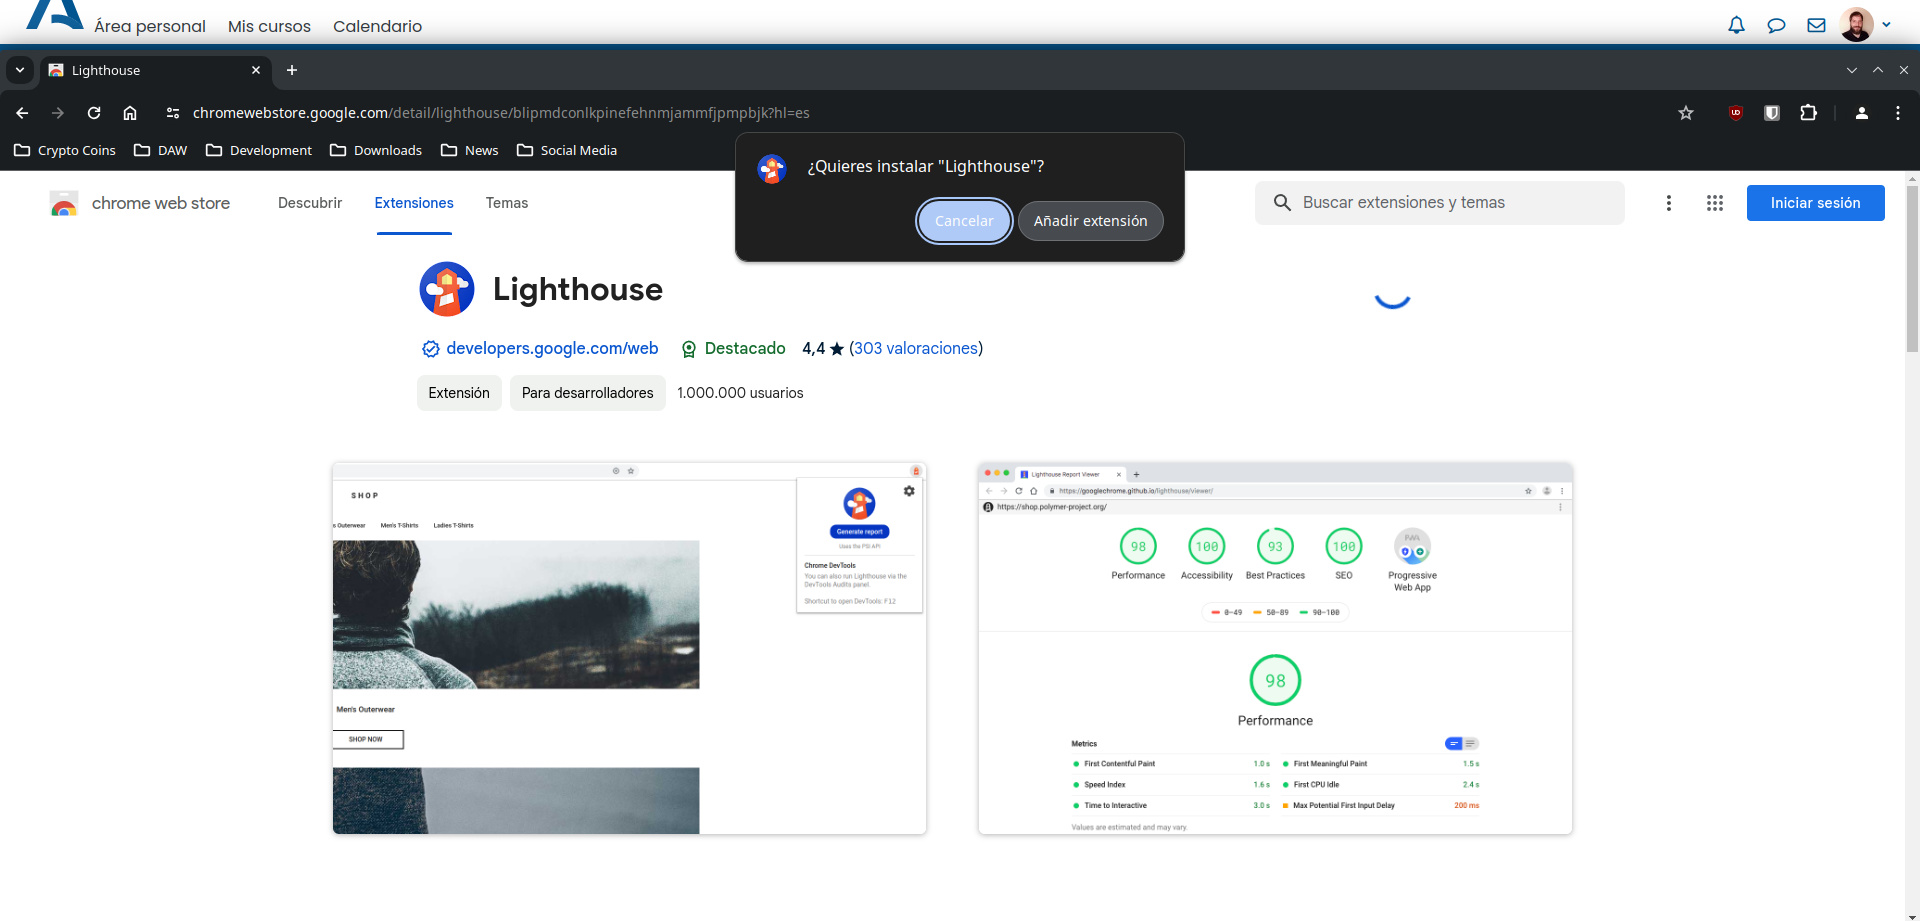
\includegraphics[scale=0.27]{lh-install.png}
        \caption{Instalación de Lighthouse en Google Chrome}
    \end{figure}

    \item En el siguiente paso se han realizado dos análisis sobre el la web del supermercado \href{https://www.mercadona.es/}{Mercadona}. El primer análisis se ha realizado de forma normal, como podemos ver en la siguiente captura de pantalla.

    \begin{figure}[H]
        \centering
        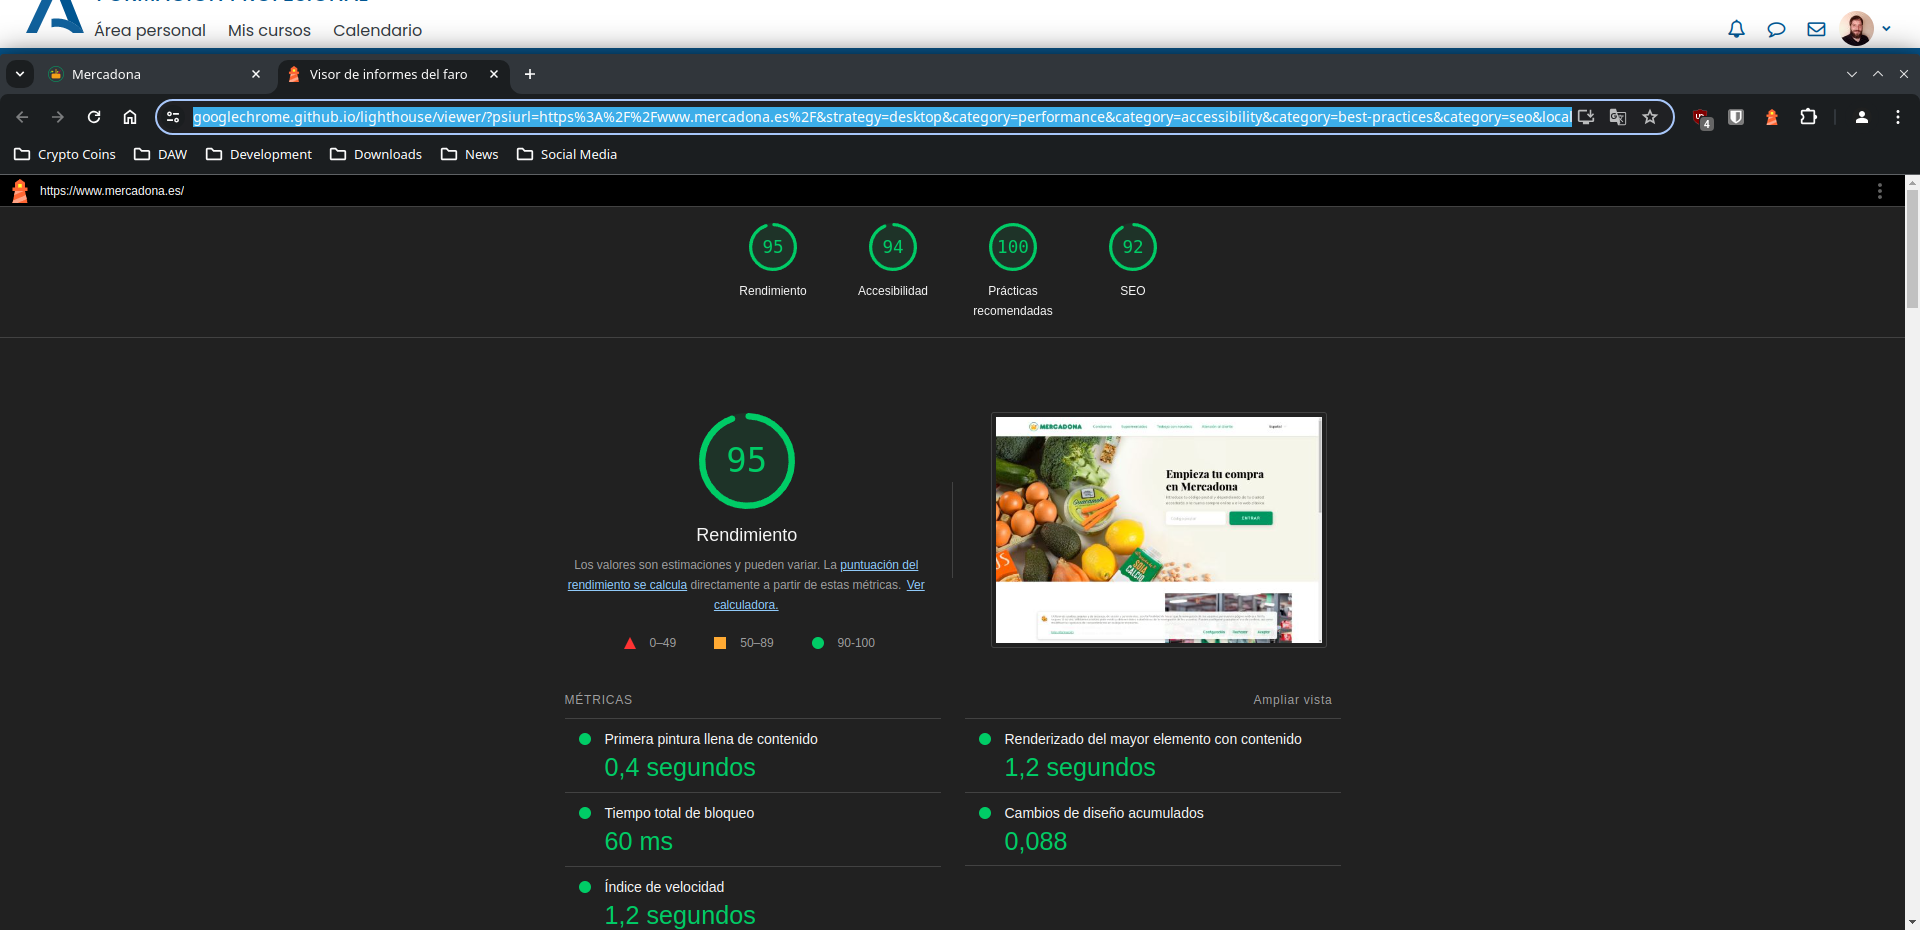
\includegraphics[scale=0.27]{lh-merca-1.png}
        \caption{Análisis de la web de Mercadona en modo normal}
    \end{figure}

    \item El siguiente paso ha sido realizar el mismo análisis, pero en este caso, se ha realizado con el navegador en \textbf{modo incógnito}. A diferencia del punto anterior, en el que se ha realizado directamente el análisis desde la extensión, en este caso se ha realizado el análisis desde las \textbf{Devtools} de Google Chrome.

    Como podemos ver en la siguiente captura, el valor que se ha obtenido en la \textbf{performance} ha sido bastante inferior al que se ha obtenido en modo normal. En los otros parámetros no ha habido cambios significativos, como podemos ver en la siguiente captura.

    \begin{figure}[H]
        \centering
        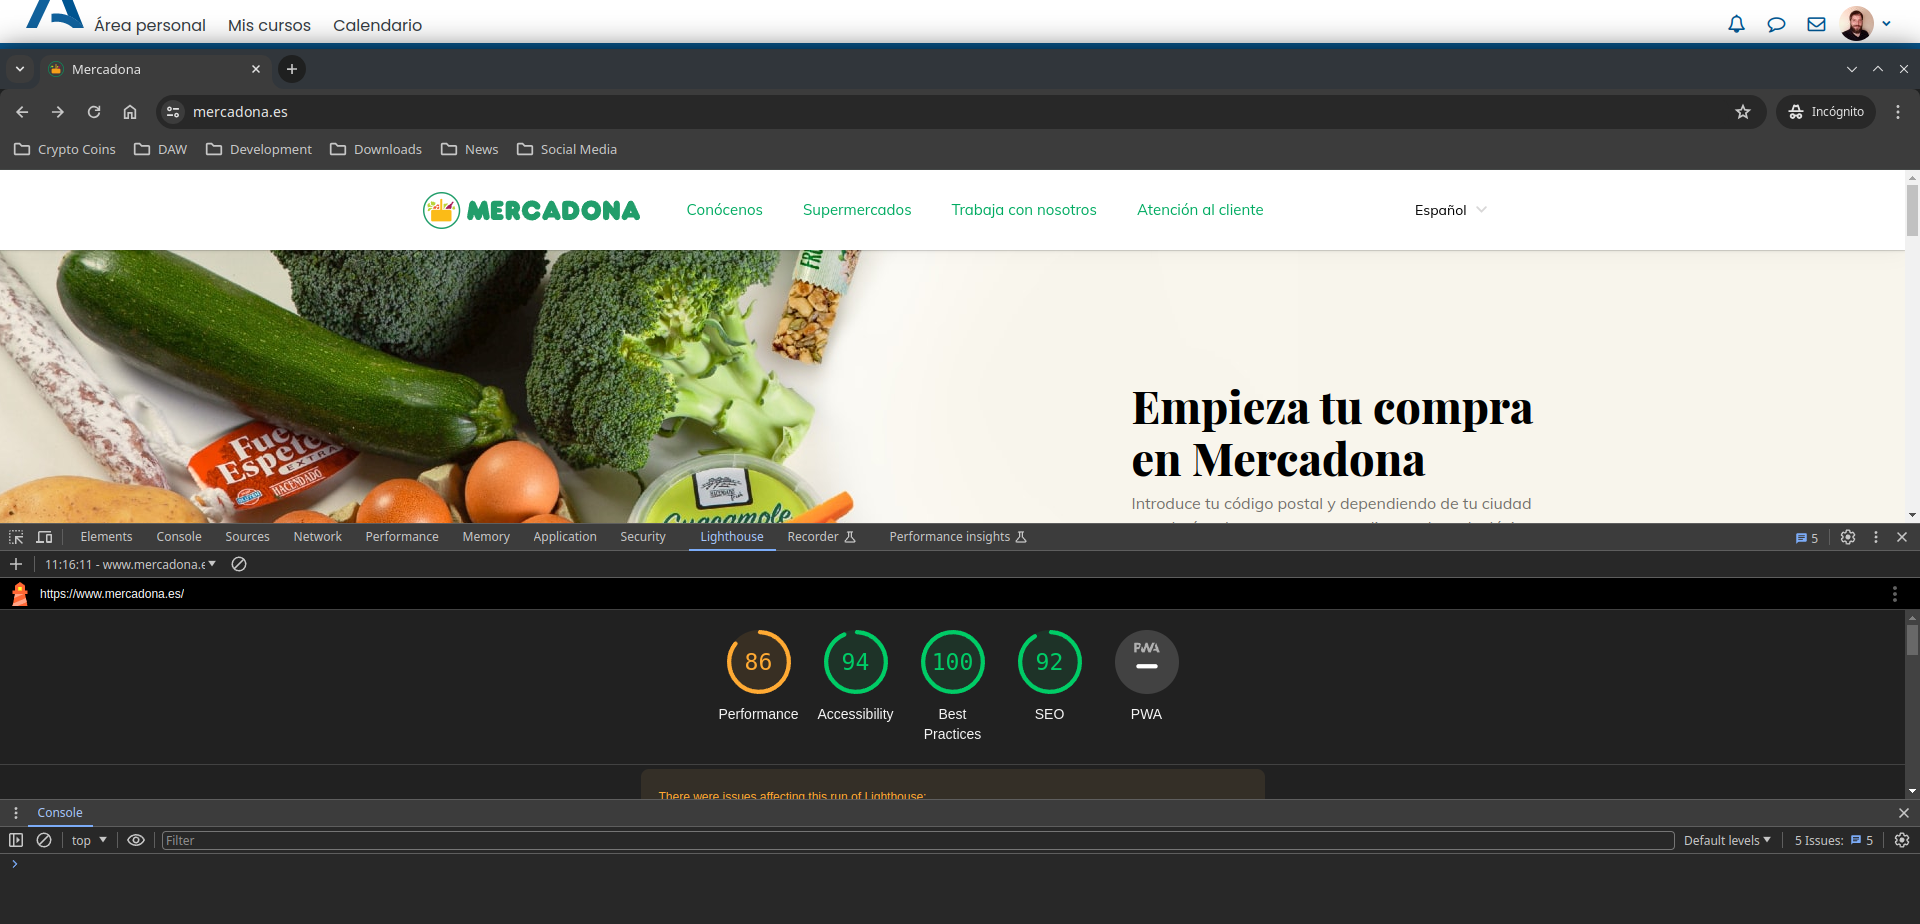
\includegraphics[scale=0.27]{lh-merca-2.png}
        \caption{Análisis de la web de Mercadona en modo incógnito}
    \end{figure}

    \item La \textbf{puntuación} global obtenida ha sido de \textbf{95}. Si atendemos a las puntuación específicas de cada parámetro , estás han sido las siguientes:

    \begin{itemize}
        \item \textbf{Rendimiento}: 95
        \item \textbf{Accesibilidad}: 94
        \item \textbf{Prácticas Recomendadas}: 100
        \item \textbf{SEO}: 92
    \end{itemize}

    \item En el informe que se ha generado, hay un montón de \textbf{recomendaciones} para mejorar el rendimiento de la web. Se han escogido
    la 3 primeras por ser las más relevantes, y que son las siguientes:

    \begin{itemize}
        \item \textbf{Reducir el contenido de Javascript que no se utiliza}: esta sugerencia nos insta a que reduzcamos el código de javascript que no se utiliza o a posponer la carga de este contenido hasta que sea necesaria su utilización. En el texto también se nos indica como podemos posponer la carga de script si no vamos a renderizar en el servidor mediante el uso de React.lazy() y algunas librerías de terceros.

        \item \textbf{Imágenes públicas con formato de nueva generación}: como se nos muestra en una lista de imágenes, se usan bastantes con el formato \textbf{JPEG}, recomendándonos cambiar dicho formato a alguno más nuevo, como WEBP, ya que realizan mejores compresiones de la imagen manteniendo una calidad incluso superior.

        \item \textbf{Evitar usar Javascript antiguo en navegadores modernos}: los polyfills y transform ayudan a que navegadores antiguos usen funcionalidades modernas de Javascript, pero es recomendable realizar detección de funcionalidades en el navegador y no cargar estos contenidos de Javascript si no son necesarios.
    \end{itemize}
\end{itemize}

\section{Ejercicio 3: Trabajando con PageSpeed Insights de Google}
Esta herramienta permite conocer en pocos segundos los problemas de la web tanto para móvil como para ordenador, aportando soluciones a dichos problemas. Obtiene también una puntuación basada en los datos que proporciona la ejecución de Lighthouse.

\begin{itemize}
    \item Realiza un  informe  que deberá contener los problemas de carga que se encuentran y las acciones que realizarías para mejorar la carga de la página.
    \item Distingue en el informe los problemas que encuentra por un lado para móvil y por otro lado para web
\end{itemize}

\subsection{Solución}

En este aparado vamos a usar la herramienta \textbf{PageSpeed Insights} de Google para comprobar el rendimiento de la web y los diferentes problemas que tiene.

\begin{itemize}
    \item En primer lugar se ha realizado en la página de PageSpeed Insights el análisis de la web del supermercado  \href{https://www.mercadona.es/}{Mercadona}, para continuar realizándolo con la misma página que en el apartado anterior. En las siguientes capturas podemos ver el resultado del diagnóstico para la carga de la web en ordenadores y dispositivos móviles.

    \begin{figure}[H]
        \centering
        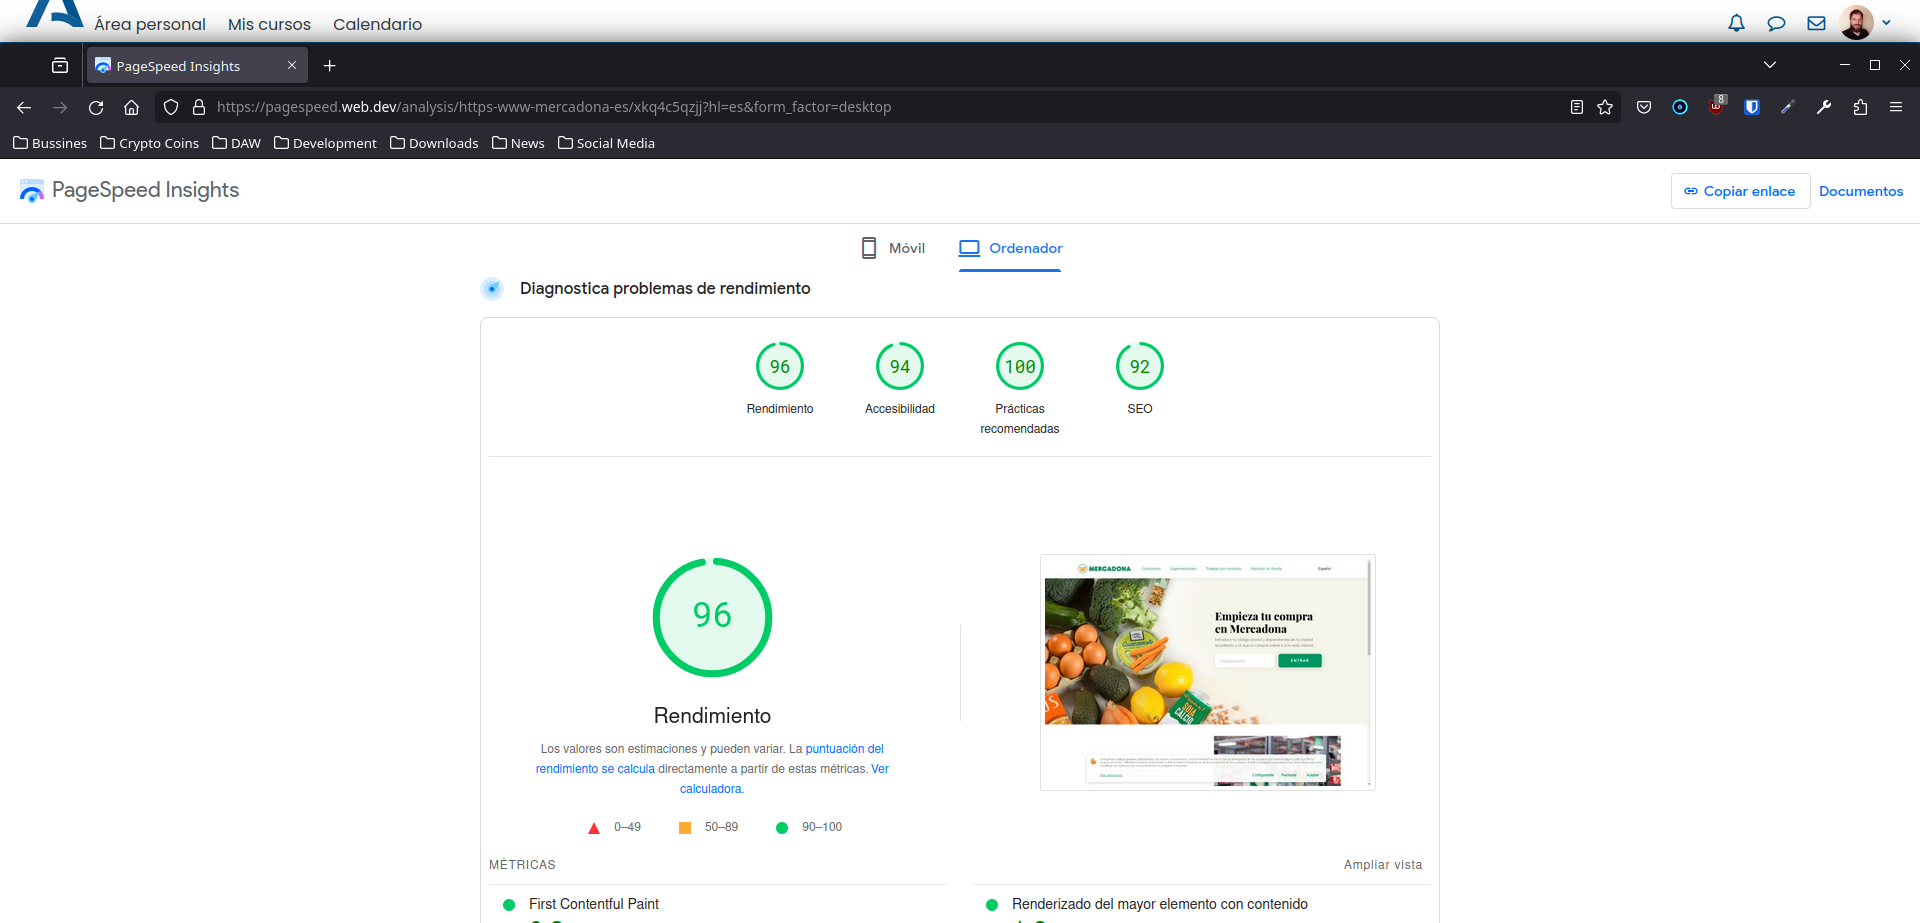
\includegraphics[scale=0.26]{page-1.png}
        \caption{Resultado de PageSpeed Insights para la carga en ordenador}
    \end{figure}

        \begin{figure}[H]
        \centering
        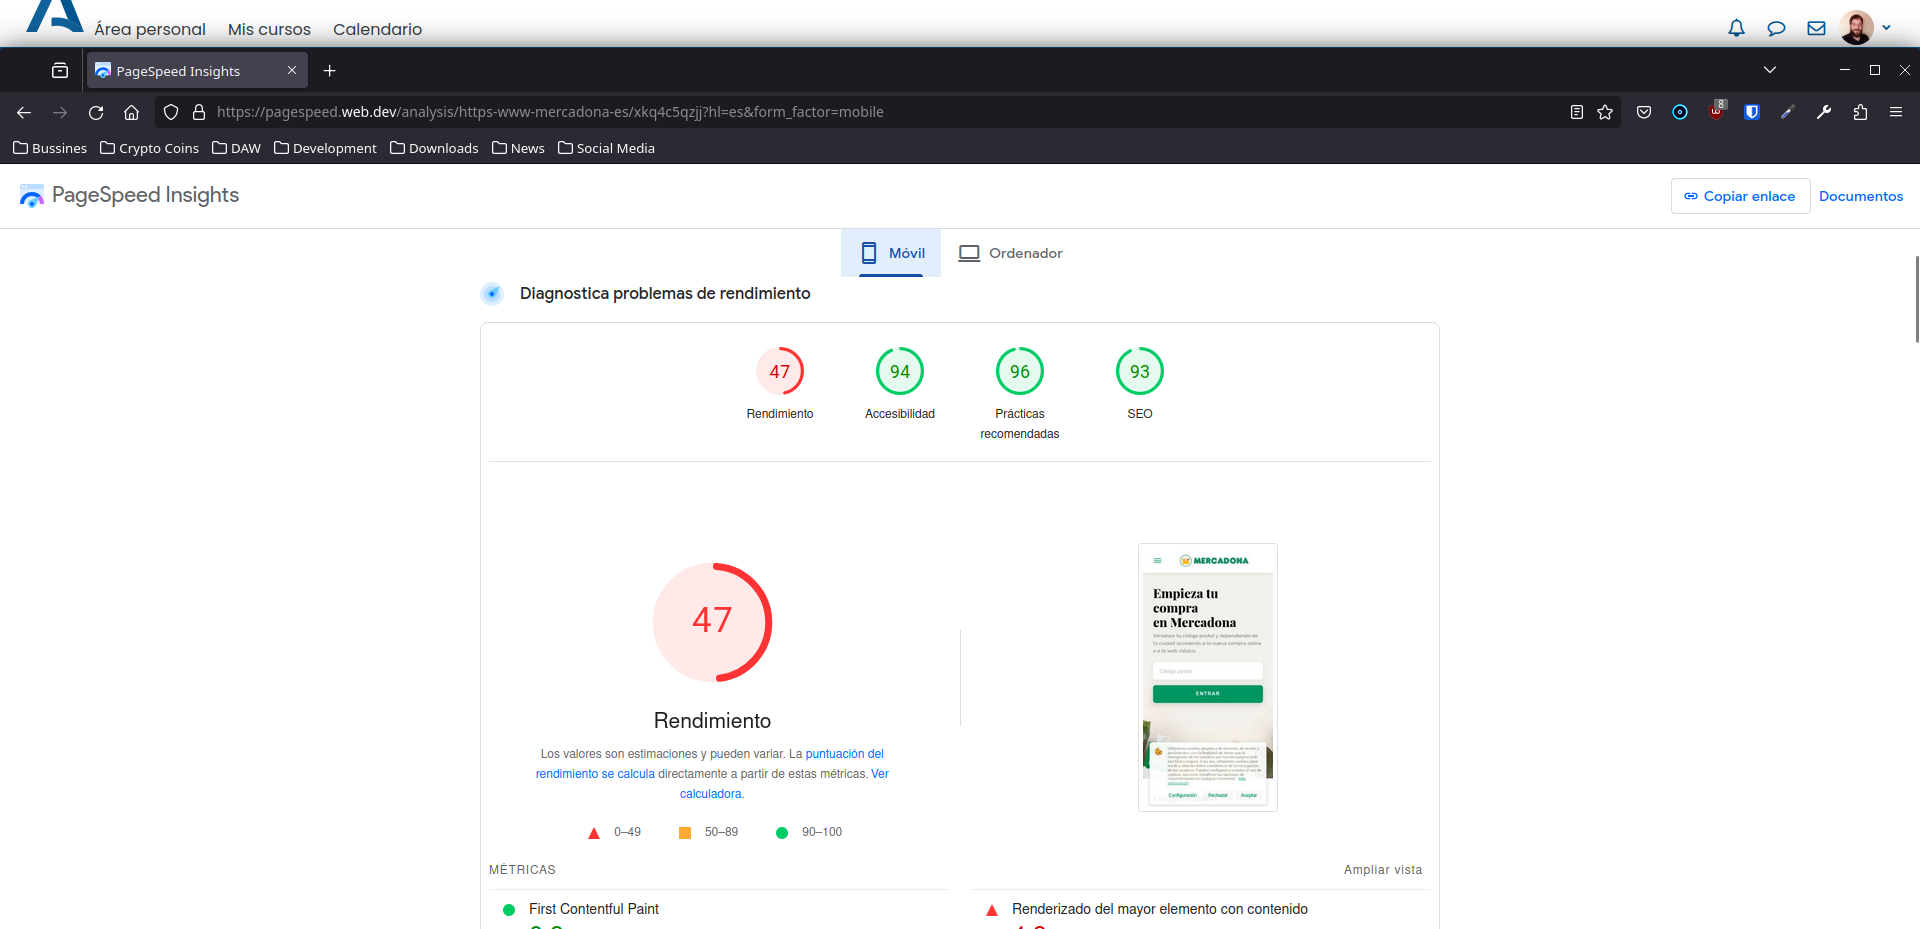
\includegraphics[scale=0.26]{page-2.png}
        \caption{Resultado de PageSpeed Insights para la carga en móviles}
    \end{figure}
\end{itemize}

Como podemos ver en las capturas, la puntuación obtenida para la versión de ordenador es muy similar a la de Lighthouse, en cambio la versión de móvil tiene más problemas. En el siguiente punto vamos a ver algunos de ellos para cada una de las versiones.

\begin{itemize}
    \item Los \textbf{principales problemas} que se han encontrado para cada una de las versiones de la página web son los siguientes:

    \begin{itemize}
        \item \textbf{Versión de Ordenador}: en este aspecto, los problemas son muy similares a los que se han encontrado con Lighthouse, aunque se han obtenido una puntuación superior a \textbf{90} en todos los parámetros analizados, como podemos ver en la siguiente captura.

        \begin{figure}[H]
            \centering
            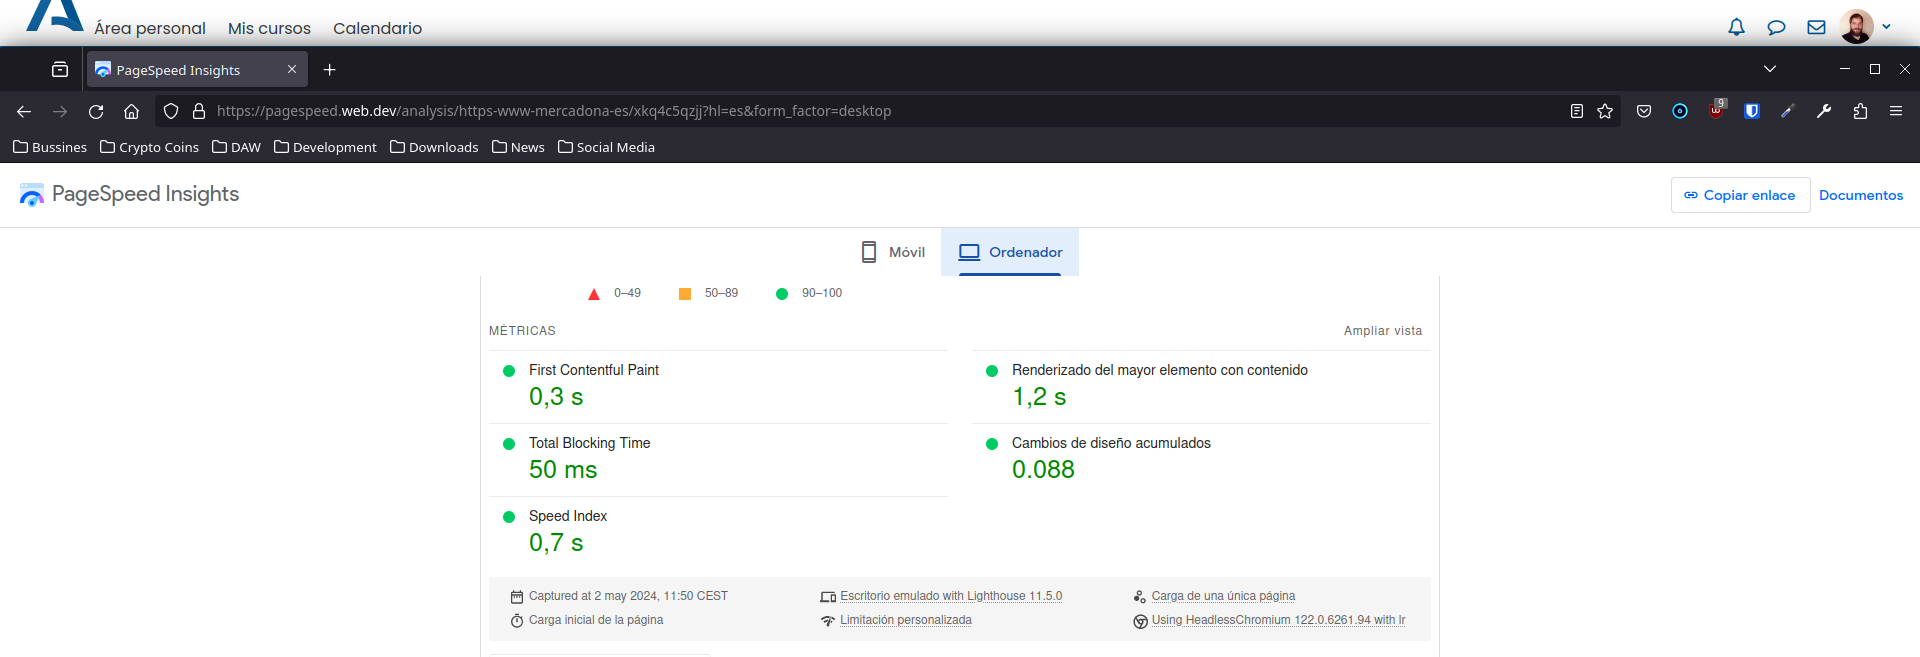
\includegraphics[scale=0.26]{met-1.png}
            \caption{Métricas de la versión de la web para ordenadores}
        \end{figure}

        Respecto a las sugerencias que nos hemos encontrado para mejorar el rendimiento en ordenadores, podemos encontrar la siguientes, que se van a enumerar:

        \begin{itemize}
            \item Publica imágenes con \textbf{formatos de nueva generación}.
            \item\textbf{Reduce el contenido de Javascript} que no se utilice.
            \item \textbf{Precargar la imagen de renderizado} del mayor elemento con contenido
            \item Los elementos de imagen no tienen \textbf{width ni height explícitos}.
        \end{itemize}
    \end{itemize}

    Algunas de estas recomendaciones han coincidido con las de Lighthouse, mientras que otras son nuevas ya que los parámetros empleados
    no son solo los de laboratorio, sino los del uso real de la web por un usuario.

    \item \textbf{Versión de Móvil}: los datos obtenidos para la versión móvil han sido diferentes, con una menor puntuación en varios apartados y un desempeño peor que la versión de la web para ordenadores, como podemos ver en al siguiente captura.

    \begin{figure}[H]
        \centering
        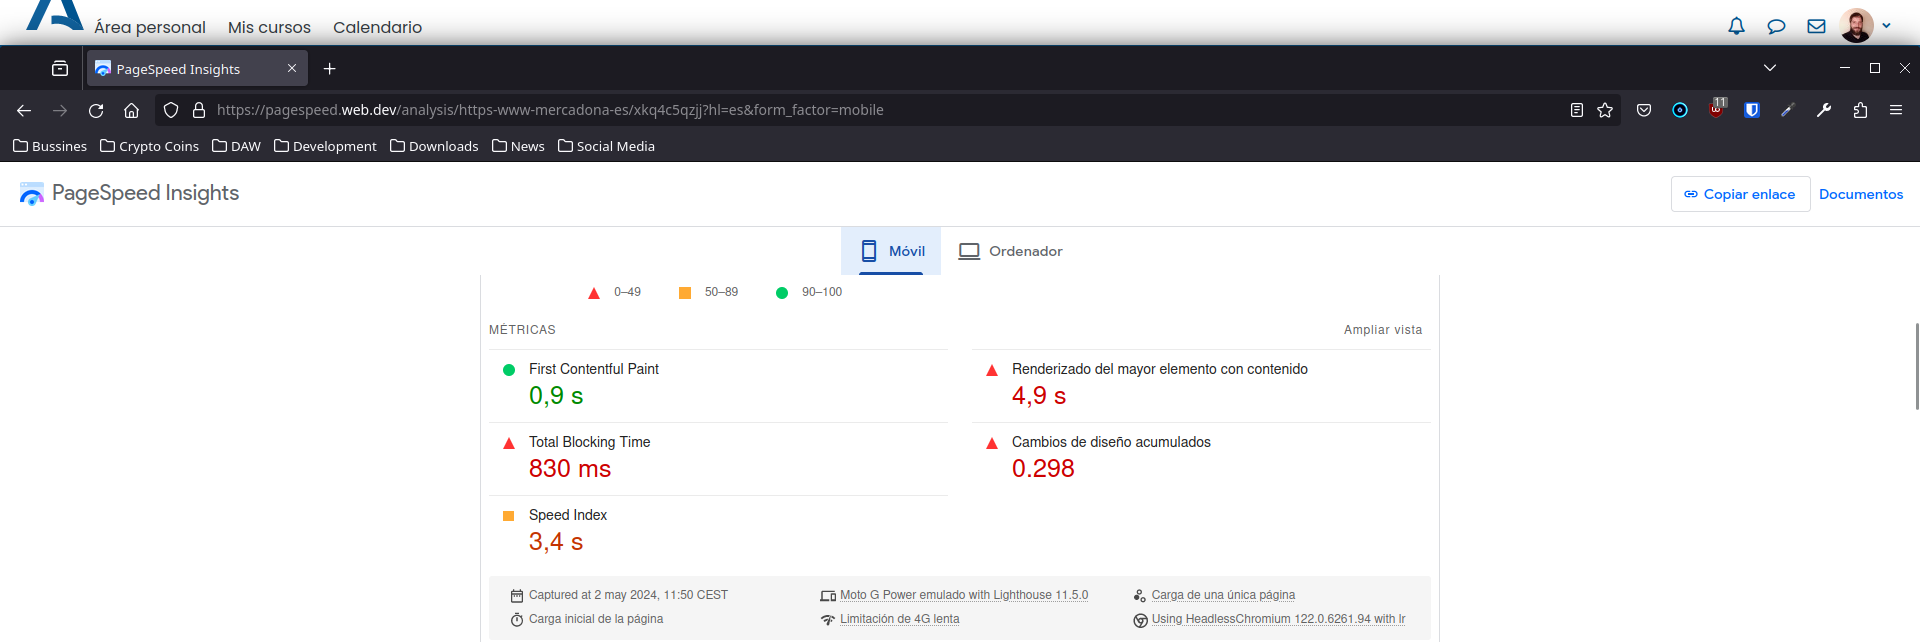
\includegraphics[scale=0.26]{met-2.png}
        \caption{Métricas de la versión de la web para móviles}
    \end{figure}

    Como vemos en la imagen anterior en la versión de móvil hay muchas métricas que se salen de los parámetros correctos, como el \textbf{tiempo de carga}, el \textbf{tiempo de bloqueo}, el \textbf{tiempo de renderizado del mayor elemento}, etc.

    Para mejorar estas métricas, algunos de las recomendaciones que nos dan son las siguientes:

    \begin{itemize}
        \item \textbf{Evitar} el \textbf{cambio de layouts}
        \item \textbf{Reducir} el \textbf{tiempo de renderizado} del mayor elemento.
        \item Publicar \textbf{imágenes} con \textbf{formatos de nueva generación}
        \item \textbf{Precargar la imagen} de renderizado del mayor elemento.
    \end{itemize}

    Como vemos, la sugerencias que se nos dan en este caso difieren de las que se nos da para la versión de la web en ordenadores.
\end{itemize}

\section{Ejercicio 4: Optimización de imágenes}
Debes realizar  3 fotos con autoría propia ( puede ser tres  que ya tengas realizadas o hacerlas una con el móvil) . NOTA: si la haces con el móvil y este es iphone debes ir a la opción cámara-formatos y quitar la opción de alta eficiencia para tomar la foto. Esto evitará la optimización por parte del móvil directamente en formato HEIF/HEVC y ponerlo al más compatible.

Una vez tengas realizadas las cuatro fotos:

\begin{enumerate}
    \item Guarda las  las imágenes en una carpeta de trabajo, fotos, y a continuación realiza los siguientes ejercicios:

    \begin{enumerate}
       \item Selecciona una imagen y comprímela sin pérdida de calidad utilizando una de las herramientas indicadas (por ejemplo, Web Resizer o Compressor.io). Guarda esta imagen comprimida en la carpeta fotos  creada para esta actividad, nombrándola como la original y añadiéndole la palabra comprimida

       \item Comprime la totalidad de las imágenes DE UNA SOLA VEZ y guárdalas dentro de la carpeta fotos en una carpeta  que se llame “imágenes comprimidas”. Para ello puedes utilizar la herramienta “optimizilla” (imagecompressor.com), el cual permite arrastrar la totalidad de las imágenes desde la carpeta donde se encuentren (o cualquier otro software que crees oportuno).
    \end{enumerate}
\end{enumerate}

\subsection{Solución}
En este aparatado se han realizado 3 fotografías y se han realizado diferentes optimizaciones sobre ellas. Las fotografías se han realizado con un dispositivo móvil sin aplicar ninguna optimización y se han incluido en la carpeta \textbf{fotos} que se adjunta con este documento. A continuación, se han realizado los siguientes ejercicio para optimizarlas.

\begin{itemize}
    \item En primer lugar, se ha seleccionado una imagen, en concreto la \textbf{\textit{original-1.jpg}}, y se ha realizado una optimización sin perdida con la herramienta \textbf{Web Resizer}.

    En este caso, la ganancia ha sido realmente pequeña, siendo de unos \textbf{10.38 KB} el disminución de peso de la imagen tras la optimización. Esto se puede deber a que el formato de la imagen original ya esta optimizado, a pesar de no haber activado las optimizaciones en el dispositivo móvil.

    En la siguiente captura podemos ver el resultado en la página de Web Resizer.

    \begin{figure}[H]
        \centering
        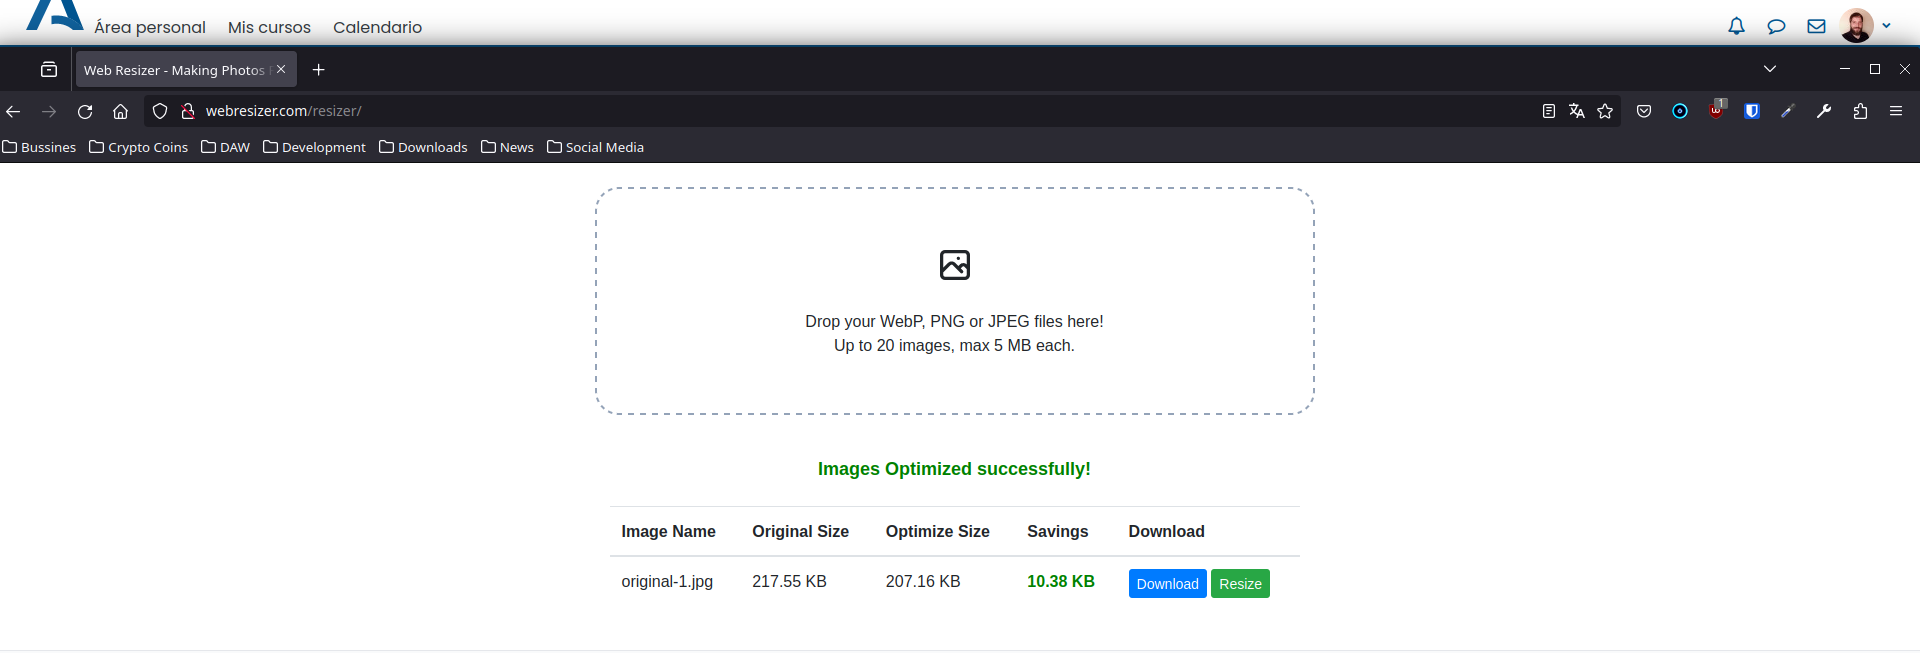
\includegraphics[scale=0.23]{imagen-1.png}
        \caption{Optimización con Web Resizer de una imagen}
    \end{figure}

    \item En segundo logar se han comprimido 3 imágenes de forma simultánea usando para ello \textbf{Optimizilla}, que como podemos ver en la siguiente captura ha optimizado las imágenes al mismo tiempo.

    \begin{figure}[H]
        \centering
        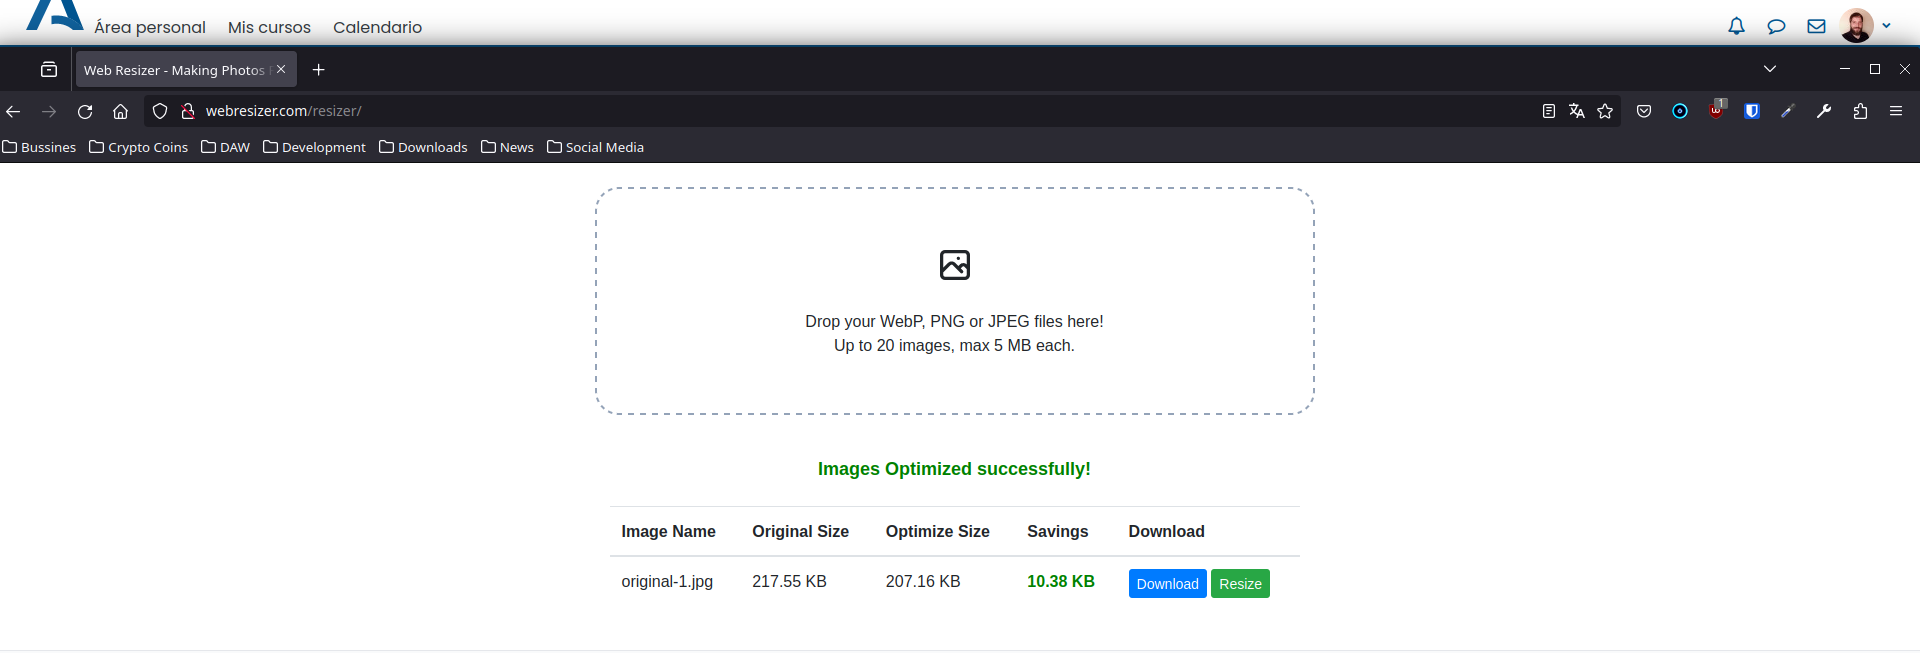
\includegraphics[scale=0.23]{imagen-1.png}
        \caption{Optimización de las 3 imágenes con Optimizilla}
    \end{figure}
\end{itemize}

% Bibliography

%\newpage
%\bibliography{citas}
%\bibliographystyle{unsrt}

\end{document}